\documentclass{standalone}
\usepackage{tikz}
\usetikzlibrary{patterns, positioning}

\begin{document}
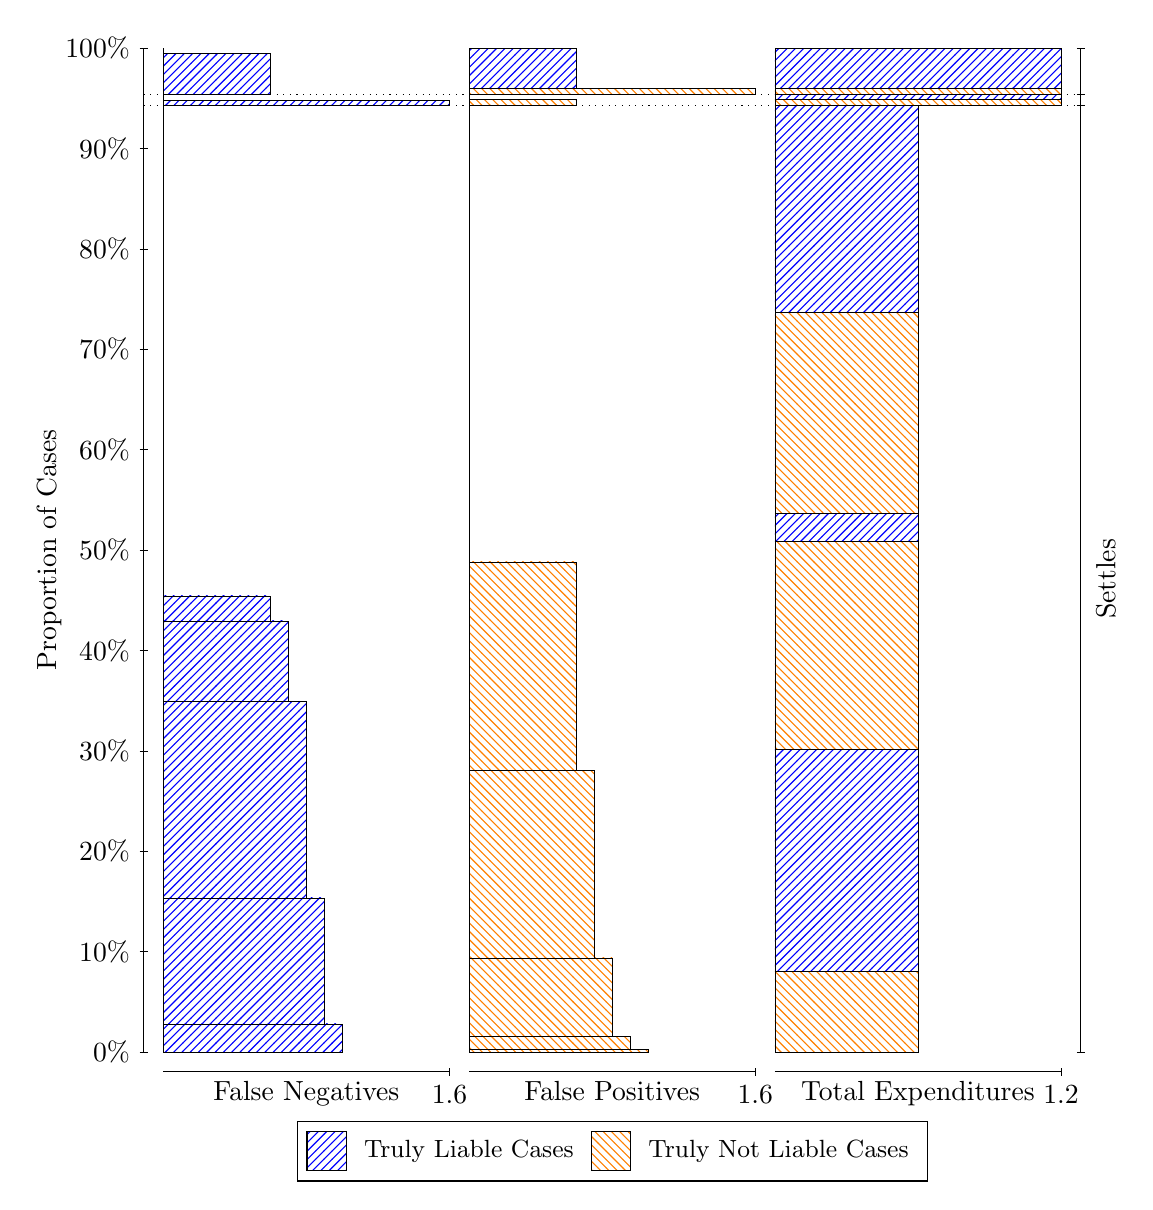
\begin{tikzpicture}
\draw[black, very thin] (1.5,1.75) -- (1.5,14.5);
\node[rotate=90, anchor=center] at (0.3, 8.125) {Proportion of Cases};
\draw[black, very thin] (1.45,1.75) -- (1.55,1.75);
\node[anchor=east] at (1.45, 1.75) {0\%};
\draw[black, very thin] (1.45,3.025) -- (1.55,3.025);
\node[anchor=east] at (1.45, 3.025) {10\%};
\draw[black, very thin] (1.45,4.3) -- (1.55,4.3);
\node[anchor=east] at (1.45, 4.3) {20\%};
\draw[black, very thin] (1.45,5.575) -- (1.55,5.575);
\node[anchor=east] at (1.45, 5.575) {30\%};
\draw[black, very thin] (1.45,6.85) -- (1.55,6.85);
\node[anchor=east] at (1.45, 6.85) {40\%};
\draw[black, very thin] (1.45,8.125) -- (1.55,8.125);
\node[anchor=east] at (1.45, 8.125) {50\%};
\draw[black, very thin] (1.45,9.4) -- (1.55,9.4);
\node[anchor=east] at (1.45, 9.4) {60\%};
\draw[black, very thin] (1.45,10.675) -- (1.55,10.675);
\node[anchor=east] at (1.45, 10.675) {70\%};
\draw[black, very thin] (1.45,11.95) -- (1.55,11.95);
\node[anchor=east] at (1.45, 11.95) {80\%};
\draw[black, very thin] (1.45,13.225) -- (1.55,13.225);
\node[anchor=east] at (1.45, 13.225) {90\%};
\draw[black, very thin] (1.45,14.5) -- (1.55,14.5);
\node[anchor=east] at (1.45, 14.5) {100\%};

\draw[black, very thin] (13.4,1.75) -- (13.4,14.5);
\draw[black, very thin] (13.35,1.75) -- (13.45,1.75);
\node[anchor=west] at (13.35, 1.75) {};
\draw[black, very thin] (13.35,13.767) -- (13.45,13.767);
\node[anchor=west] at (13.35, 13.767) {};
\draw[black, very thin] (13.35,13.914) -- (13.45,13.914);
\node[anchor=west] at (13.35, 13.914) {};
\draw[black, very thin] (13.35,14.5) -- (13.45,14.5);
\node[anchor=west] at (13.35, 14.5) {};

\draw[black, very thin, pattern color=blue, pattern=north east lines] (1.75,1.75) rectangle (4.0208,2.1071);
\draw[black, very thin, pattern color=blue, pattern=north east lines] (1.75,2.1071) rectangle (3.7937,3.7065);
\draw[black, very thin, pattern color=blue, pattern=north east lines] (1.75,3.7065) rectangle (3.5667,6.2018);
\draw[black, very thin, pattern color=blue, pattern=north east lines] (1.75,6.2018) rectangle (3.3396,7.2235);
\draw[black, very thin, pattern color=blue, pattern=north east lines] (1.75,7.2235) rectangle (3.1125,7.5412);
\draw[black, very thin, pattern color=orange, pattern=north west lines] (1.75,7.5412) rectangle (1.75,13.767);
\draw[black, very thin, pattern color=blue, pattern=north east lines] (1.75,13.767) rectangle (5.3833,13.837);
\draw[black, very thin, pattern color=orange, pattern=north west lines] (1.75,13.837) rectangle (1.75,13.914);
\draw[black, very thin, pattern color=blue, pattern=north east lines] (1.75,13.914) rectangle (3.1125,14.427);
\draw[black, very thin, pattern color=orange, pattern=north west lines] (1.75,14.427) rectangle (1.75,14.5);
\draw[black, very thin, pattern color=orange, pattern=north west lines] (5.6333,1.75) rectangle (7.9042,1.7828);
\draw[black, very thin, pattern color=orange, pattern=north west lines] (5.6333,1.7828) rectangle (7.6771,1.951);
\draw[black, very thin, pattern color=orange, pattern=north west lines] (5.6333,1.951) rectangle (7.45,2.9438);
\draw[black, very thin, pattern color=orange, pattern=north west lines] (5.6333,2.9438) rectangle (7.2229,5.3302);
\draw[black, very thin, pattern color=orange, pattern=north west lines] (5.6333,5.3302) rectangle (6.9958,7.9754);
\draw[black, very thin, pattern color=blue, pattern=north east lines] (5.6333,7.9754) rectangle (5.6333,13.767);
\draw[black, very thin, pattern color=orange, pattern=north west lines] (5.6333,13.767) rectangle (6.9958,13.843);
\draw[black, very thin, pattern color=blue, pattern=north east lines] (5.6333,13.843) rectangle (5.6333,13.914);
\draw[black, very thin, pattern color=orange, pattern=north west lines] (5.6333,13.914) rectangle (9.2667,13.987);
\draw[black, very thin, pattern color=blue, pattern=north east lines] (5.6333,13.987) rectangle (6.9958,14.5);
\draw[black, very thin, pattern color=orange, pattern=north west lines] (9.5167,1.75) rectangle (11.333,2.7756);
\draw[black, very thin, pattern color=blue, pattern=north east lines] (9.5167,2.7756) rectangle (11.333,5.5887);
\draw[black, very thin, pattern color=orange, pattern=north west lines] (9.5167,5.5887) rectangle (11.333,8.2339);
\draw[black, very thin, pattern color=blue, pattern=north east lines] (9.5167,8.2339) rectangle (11.333,8.5909);
\draw[black, very thin, pattern color=orange, pattern=north west lines] (9.5167,8.5909) rectangle (11.333,11.146);
\draw[black, very thin, pattern color=blue, pattern=north east lines] (9.5167,11.146) rectangle (11.333,13.767);
\draw[black, very thin, pattern color=orange, pattern=north west lines] (9.5167,13.767) rectangle (13.15,13.843);
\draw[black, very thin, pattern color=blue, pattern=north east lines] (9.5167,13.843) rectangle (13.15,13.914);
\draw[black, very thin, pattern color=orange, pattern=north west lines] (9.5167,13.914) rectangle (13.15,13.987);
\draw[black, very thin, pattern color=blue, pattern=north east lines] (9.5167,13.987) rectangle (13.15,14.5);
\draw[black, dotted] (1.5,13.767) -- (13.4,13.767);
\draw[black, dotted] (1.5,13.914) -- (13.4,13.914);
\draw[black, very thin] (1.75,1.5) -- (5.3833,1.5);
\node[anchor=north] at (3.5667, 1.5) {False Negatives};
\draw[black, very thin] (5.3833,1.45) -- (5.3833,1.55);
\node[anchor=north] at (5.3833, 1.45) {1.6};

\draw[black, very thin] (5.6333,1.5) -- (9.2667,1.5);
\node[anchor=north] at (7.45, 1.5) {False Positives};
\draw[black, very thin] (9.2667,1.45) -- (9.2667,1.55);
\node[anchor=north] at (9.2667, 1.45) {1.6};

\draw[black, very thin] (9.5167,1.5) -- (13.15,1.5);
\node[anchor=north] at (11.333, 1.5) {Total Expenditures};
\draw[black, very thin] (13.15,1.45) -- (13.15,1.55);
\node[anchor=north] at (13.15, 1.45) {1.2};

\node[black, centered, rotate=90] at (13.72, 7.7583) {Settles};



\draw (7.449999999999999,1.5) node[draw=none] (baseCoordinate) {};
\begin{scope}[align=center]
        \matrix[scale=0.5, draw=black, below=0.5cm of baseCoordinate, nodes={draw}, column sep=0.1cm]{
            \node[rectangle, draw, minimum width=0.5cm, minimum height=0.5cm, pattern=north east lines, pattern color=blue] {}; &
            \node[draw=none, font=\small] (B) {Truly Liable Cases}; &
            \node[rectangle, draw, minimum width=0.5cm, minimum height=0.5cm, pattern=north west lines, pattern color=orange] {}; &
            \node[draw=none, font=\small] (B) {Truly Not Liable Cases}; \\
            };
\end{scope}

\end{tikzpicture}
\end{document}